\chapter{Analytical Model and Preliminary Results}
In this chapter first a framework for the analysis that is performed is presented, later the basic model that is used for the analysis is presented and later calibrated and verified with experimental data available in the literature. Finally preliminary results are presented that will define the general view for the proposed research

\section{Analytical Model}

\subsection{Column}
This study focuses on the behavior of a Single Degree of Freedom Reinforce Concrete Column. The column is modeled as a cantilever structure as shown in \fref{fig:Structural_Model} This structure is modeled in OpenSees \cite{McKenna2010} using the $forceBeamColumn$ element \cite{Scott}. The forceBeamColumn element is used with two-point Gauss-Radau integration applied in the hinge regions and two-point Gauss integration applied on the element interior for a total of six integration points \cite{Scott}. The force based formulation requires only a single element to accurately represent the full nonlinear deformation of the member and the integration scheme selected prevents the loss of objectivity during softening response while also providing integration points at the member ends \cite{Calabrese2010},\cite{Scott}. The element requires the length of plasticity be defined at each end of the member, for which the tension based rectangular plastic hinge length is calculated using the following expresion\cite{Goodnight2013}:

\begin{equation}
    k=0.2*(Fu/Fy - 1) \leqslant 0.08
    L_{pc}=k*L_{eff} + 0.4D
    \gamma=0.33 for Single Bending
    L_{pt}=L_{pc}+\gamma*D
\end{equation}

Furthermore, the two-point Gauss-Radau integration is applied such that the end node integrations are weighted equal to the specified plastic hinge length, as illustrated in \fref{fig:Fiber_PlasticHinge}. Therefore, strains recorded at the end sections represent accurate values even in the case where deformation localizes to the ends from strain softening behavior. For the case of the cantilever column considered in this dissertation, only one hinge length is defined, and the opposite end is given an arbitrary unit length. 

\begin{figure}[htbp]
	\centering
	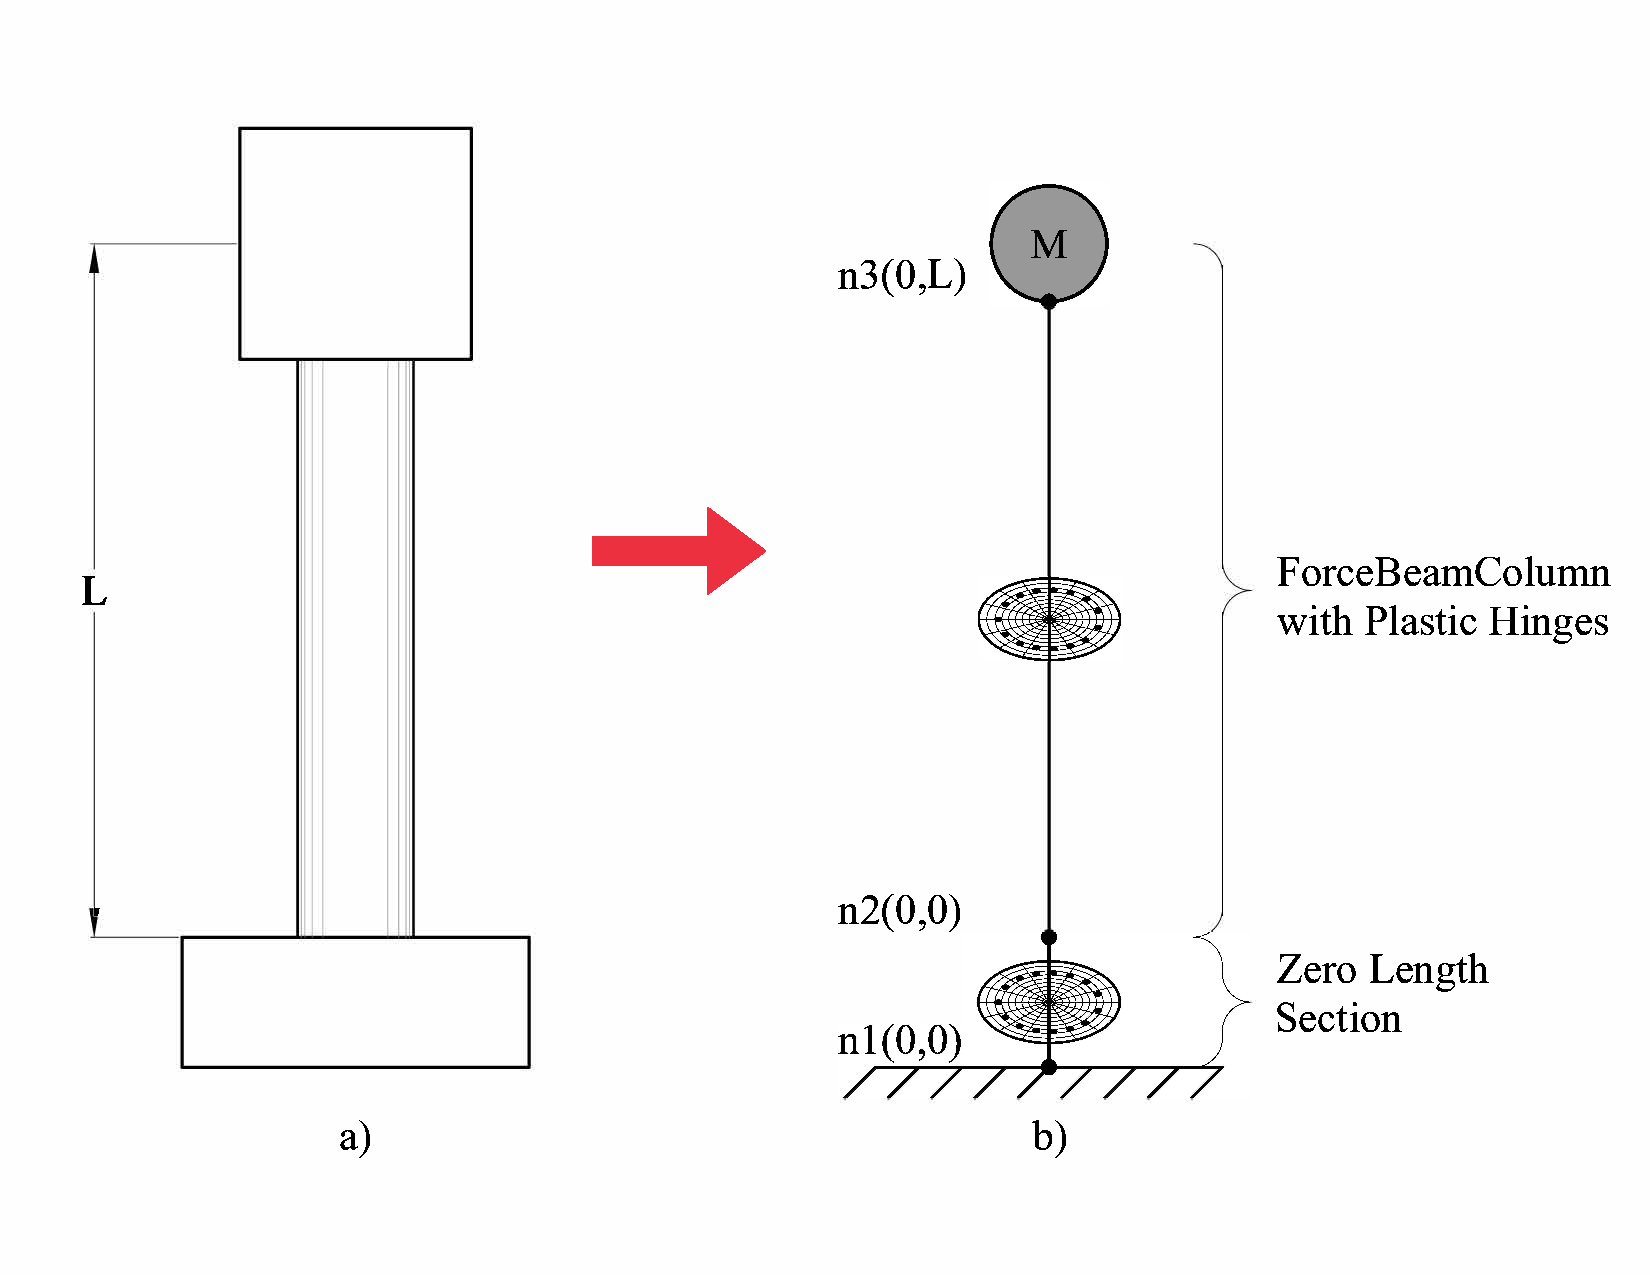
\includegraphics[width=1.0\textwidth]{Chapter-5/figs/StructuralModel_01}
	\caption{Structural Model a) SDOF Column b) Structural Model}
	\label{fig:Structural_Model}
\end{figure}

\begin{figure}[htbp]
	\centering
	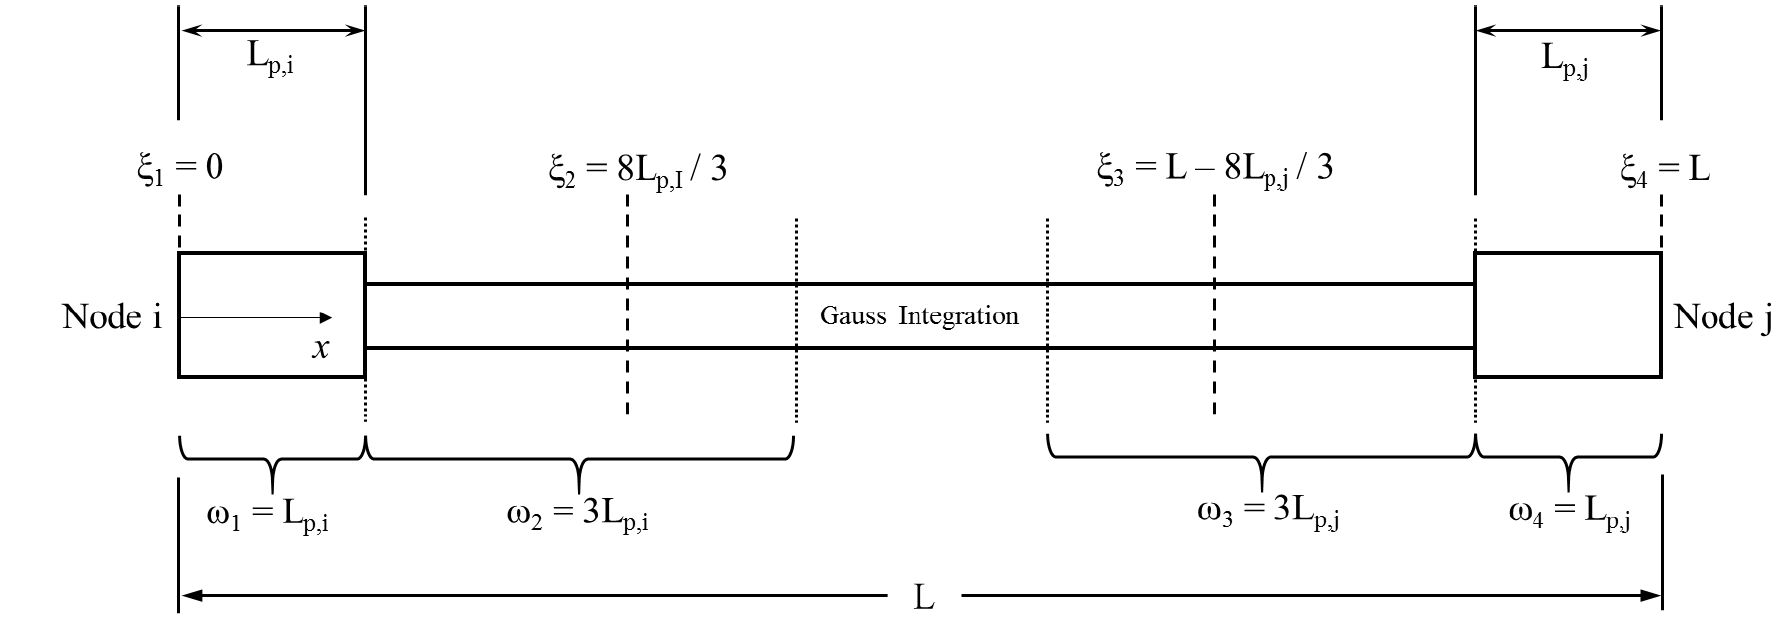
\includegraphics[width=0.9\textwidth]{Chapter-5/figs/fbc_PlasticHinge}
	\caption{End point plastic hinge method \cite{Scott}}
	\label{fig:Fiber_PlasticHinge}
\end{figure}

The section of the beam is shown in \fref{fig:ColumnSection} Two different sections are defined for use at the integration points within the element. Both sections are discretized with concrete and steel material fibers representing the geometry of the section. Concrete fibers are modeled using the $Concrete01$ material, modified for confined material strength based on the Mander confined concrete model \cite{Mander1988}. The $Steel02$ material, based on the Giuffre-Menegotto-Pinto model \cite{Filippou1983}, is used for the longitudinal reinforcement with recommended parameters ($b = 0.01, R0 = 20, cR1 = 0.925, cR2 = 0.15$). 

\begin{figure}[htbp]
	\centering
	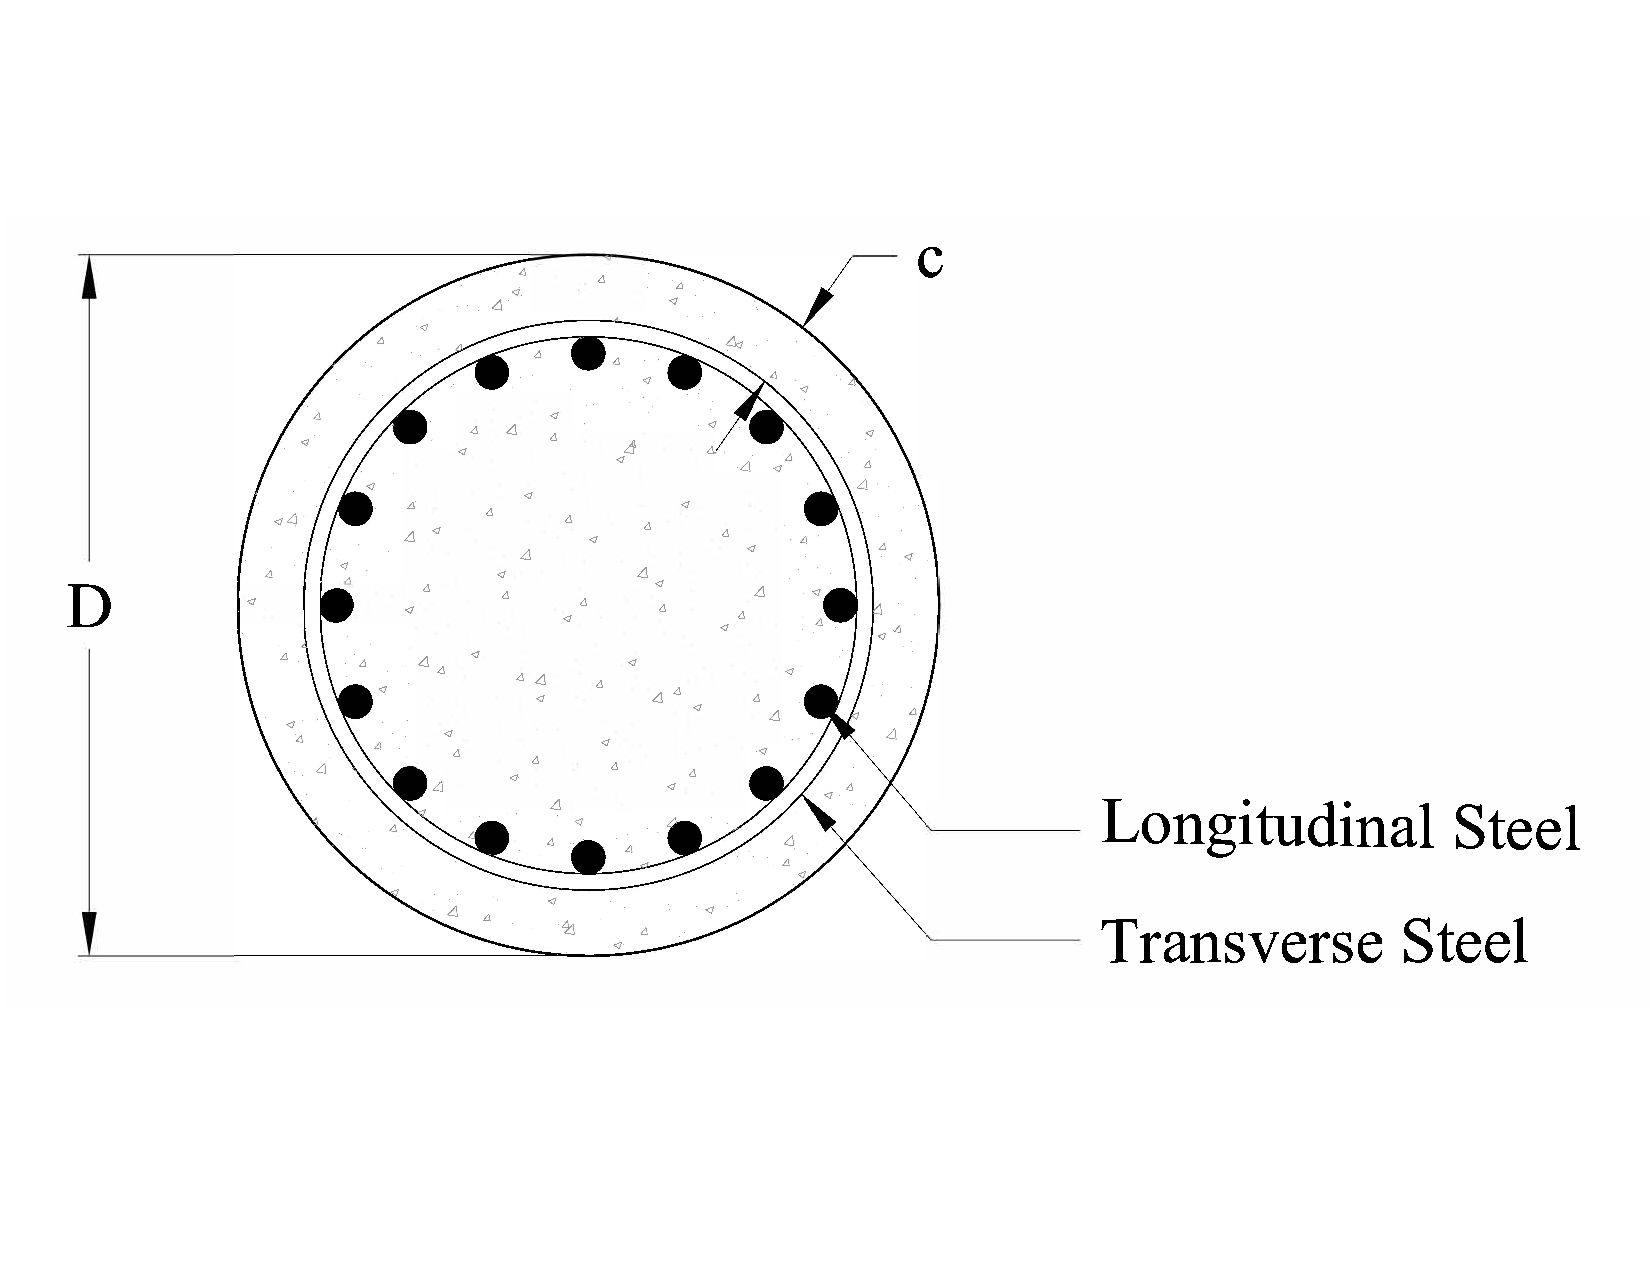
\includegraphics[width=0.7\textwidth]{Chapter-5/figs/StructuralModel_Section}
	\caption{Section of the RC Column}
	\label{fig:ColumnSection}
\end{figure}

\subsection{Strain Penetration Component}
The strain penetration is model accoording to $Bond_SP1$ material model \cite{Zhao2007}

\section{Comparison with existing physical Tests}
\subsection{pristine Condition Columns}
\lipsum[2]

\subsection{Accelerated Corrosion Columns}
\lipsum[3]

\section{Analytical Framework}

An overall analytical framework is stablished such that several analysis can be performed. From this analysis it is possible to determine the effects of damage in the performance of structures. The proposed analytical framework consists in:

\begin{enumerate}
	\item Geometrical Properties of the SDOF column 
	\item Properties of the material are evaluated (i.e. water to cement ratio, cover)
	\item For equal periods of time the Time Dependent Properties are modified
	\item Nonlinear Time History Analysis are performed for discrete events or sequence of events
	\item Results are obtained and evaluated
\end{enumerate}

This procedure has been sumarized in the form of a flow chart presented in \fref{fig:NLTHA_Framework}

\begin{figure}[htbp]
	\centering
	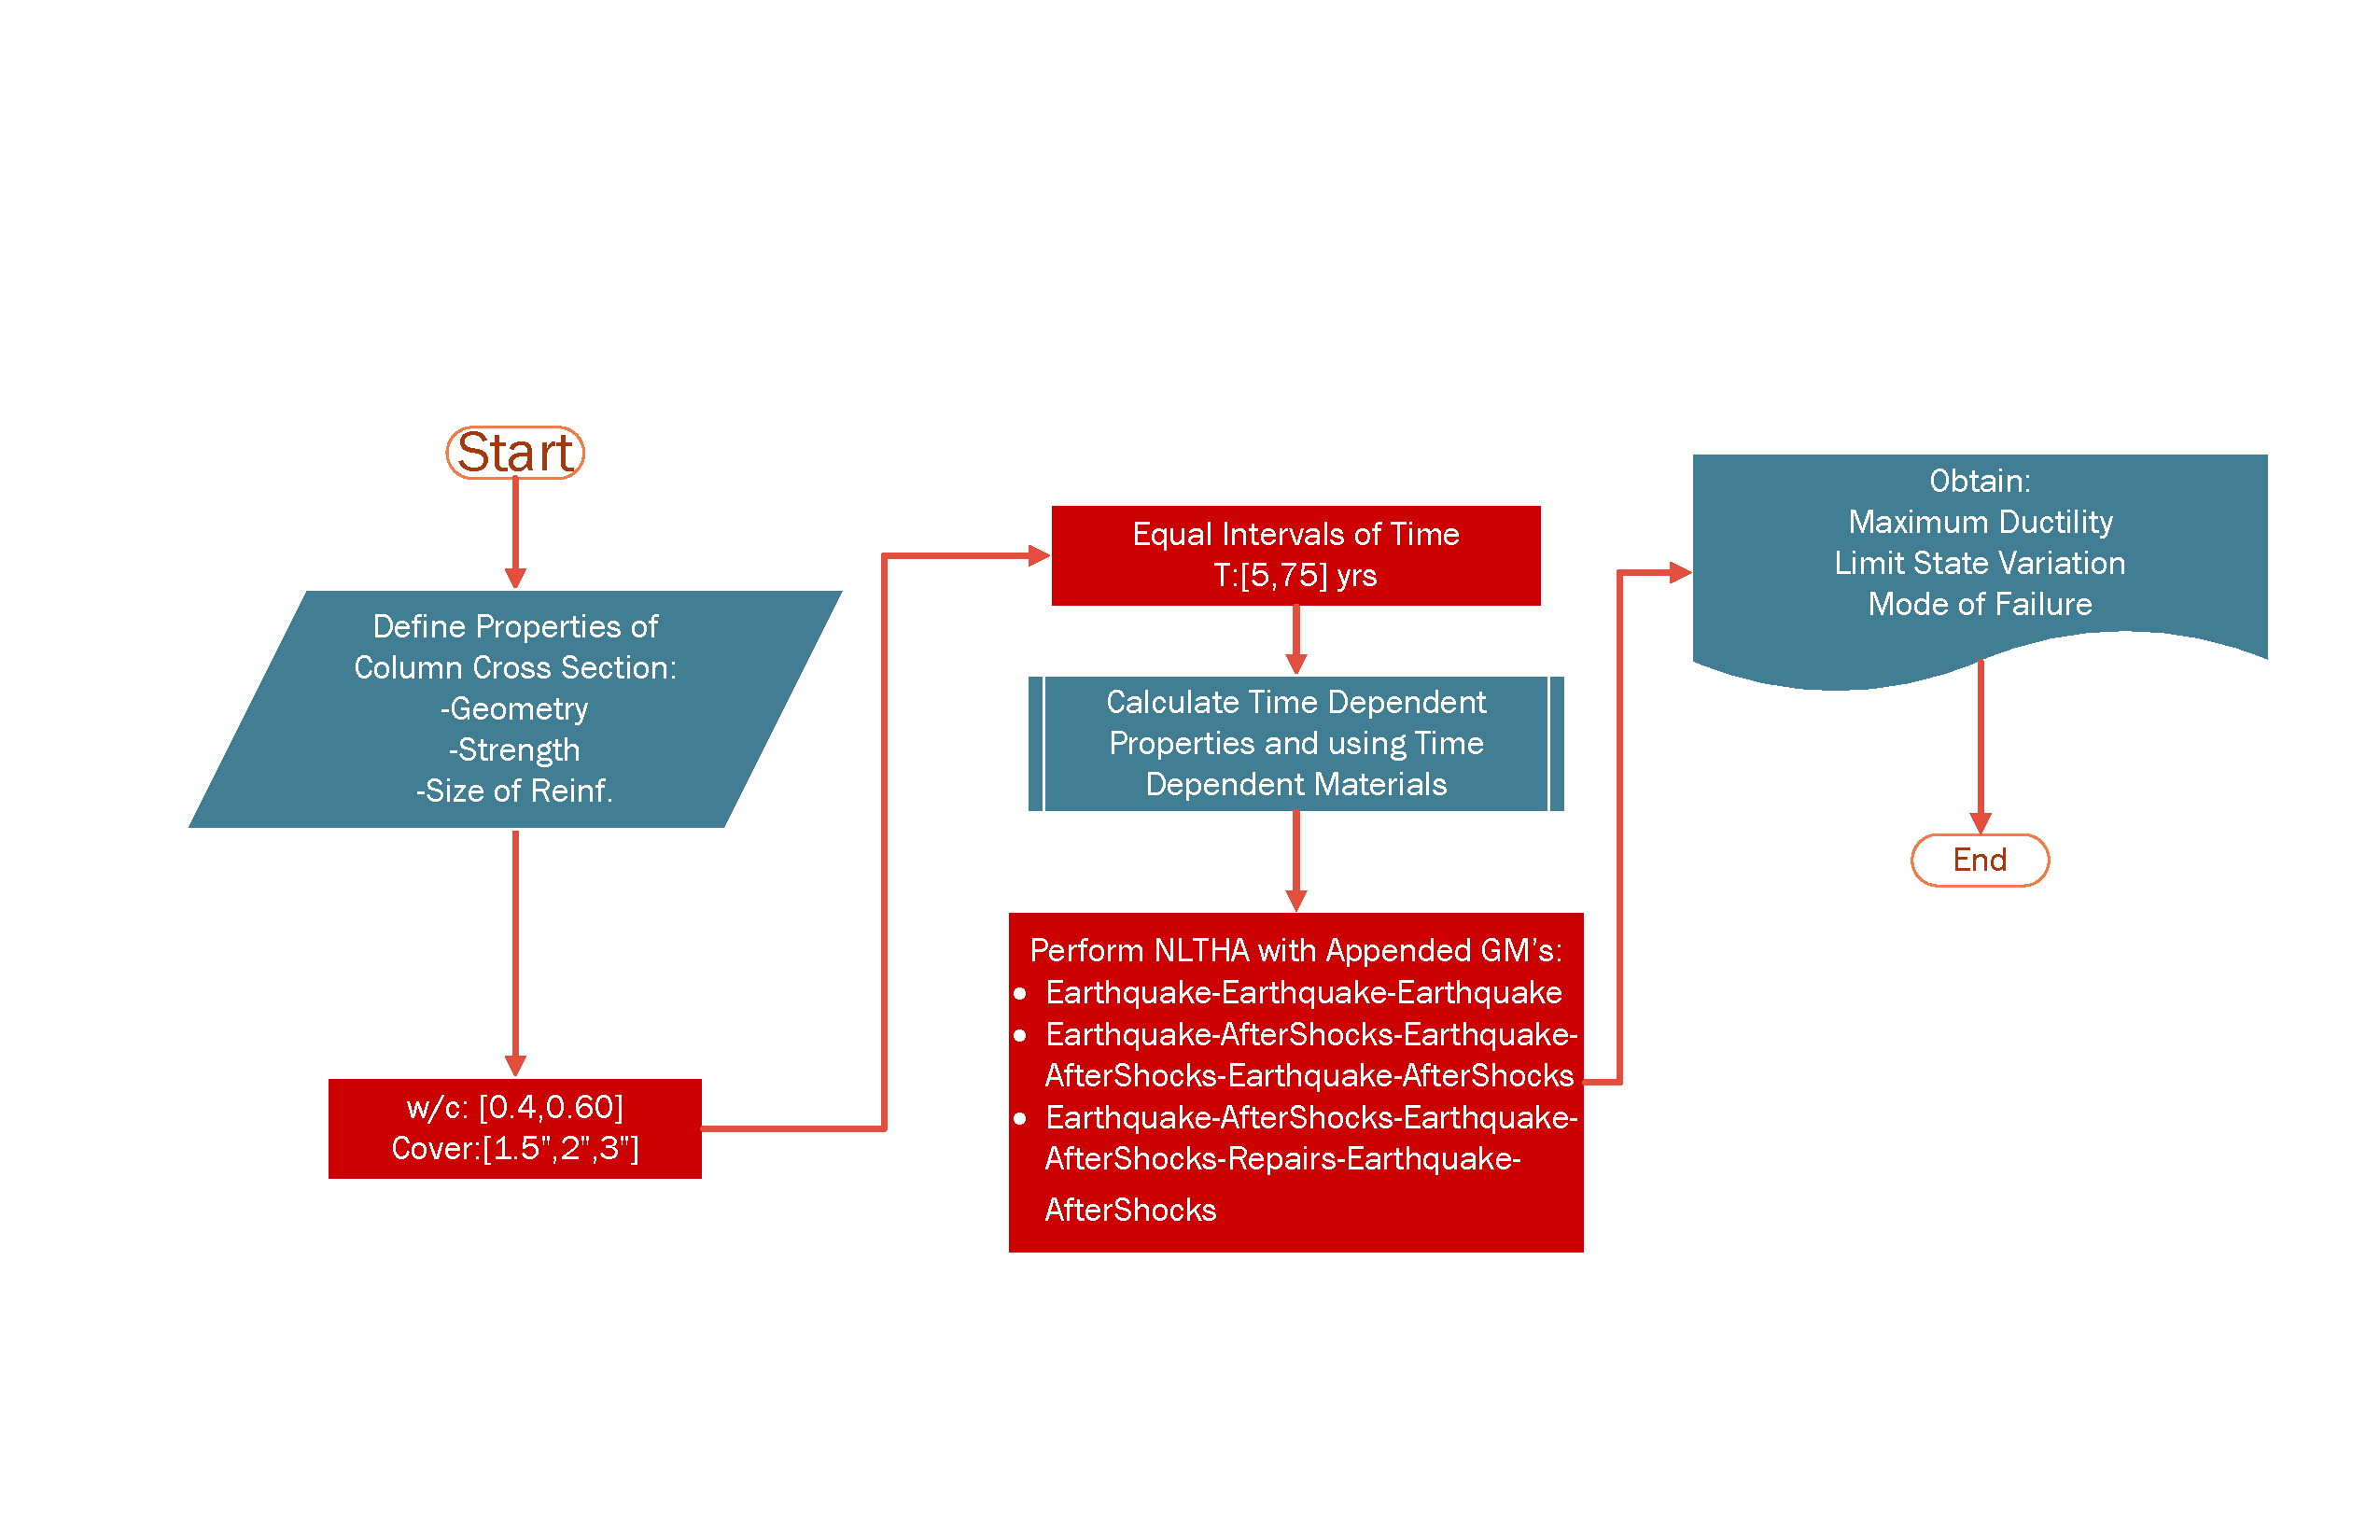
\includegraphics[width=0.9\textwidth]{Chapter-5/figs/AnalysisFramework_01}
	\caption{Analysis Framework Flowchart}
	\label{fig:NLTHA_Framework}
\end{figure}

\section{Earthquake selection}
\lipsum[4]
\section{Results from NLTHA}
\lipsum[5]
\subsection{Effect on global response}
\lipsum[6]
\subsection{Effect on local response}
\lipsum[7]
\subsection{Preliminary results}
\lipsum[8]
